\documentclass[11pt,a4paper]{article}
\usepackage[T1]{fontenc}
\usepackage[utf8]{inputenc}
\usepackage[brazilian]{babel}
\usepackage{lmodern,amsmath,amssymb,booktabs,longtable,array,enumitem,xcolor,verbatim,pdfpages}
\usepackage[margin=24mm]{geometry}
\usepackage[hidelinks]{hyperref}
\setlist{itemsep=2pt,topsep=3pt}
\setlength{\parindent}{0pt}\setlength{\parskip}{5pt}\emergencystretch=3em
\newcommand{\dd}{\,\mathrm d}
\newcommand{\ef}{e_f}
\newcommand{\nf}{n_f}
\newcommand{\Edia}{E_N^{\rm dia}}
\newcommand{\blk}[1]{\textbf{#1}}
\newenvironment{roteiro}[3]{%
  \subsection*{#1\quad{\normalfont #2}}
  \par\noindent\textit{#3}\par}{\vspace{4pt}\hrule\vspace{2pt}}
\title{\textbf{Dossiê de verificação independente}\\[2pt]
\large Parte III, Seções III.11 e III.12 — erro interpolatório diádico e lei de fase\\[2pt]
\normalsize Instruções, roteiros por item e páginas a verificar}
\author{}
\date{Volume \emph{Biblioteca determinística: volume unificado} (124 páginas)\\
repositório Walc21/Biblioteca-unificada-artigo-e-formaliza-o-Lean, \texttt{main} em \texttt{1de59e1} mais as correções do PR seguinte (branch \texttt{corrige-verificadores-e-dossie})\\
preparado em 17/11/2026}
\begin{document}
\maketitle
\thispagestyle{empty}

\section*{0.\; Como usar este dossiê}
Este arquivo tem três partes, em um só PDF.
\begin{enumerate}[leftmargin=1.6em]
\item \textbf{Instruções} (seções 1 a 5): o que se pede, as convenções do texto, o protocolo de verificação e o grafo de dependências.
\item \textbf{Roteiros por item} (seção 6): para cada teorema, lema, corolário ou observação de III.11 e III.12, uma lista de passos \emph{específicos} a verificar, casos-limite a atacar e a verificação independente sugerida.
\item \textbf{Páginas a verificar} (Apêndice A, ao final): as páginas 69 a 82 do volume, reproduzidas sem alteração. A página $k$ do apêndice é a página $68+k$ do volume, e as referências «p.~N» neste dossiê usam a numeração do volume.
\end{enumerate}
O Apêndice B traz um verificador independente (cerca de 25 linhas, só \texttt{mpmath}) e as demais rotinas do repositório.
\textbf{Ordem sugerida:} ler as seções 3 e 4; ler os itens na ordem III.11.1, III.11.3, III.12.1, III.12.2, III.12.5, III.12.6, III.12.7, III.12.8; deixar III.11.2, III.12.3, III.12.4 e III.12.9 por último.

\section{Escopo}
\begin{longtable}{@{}p{.18\linewidth}p{.07\linewidth}p{.26\linewidth}>{\footnotesize\raggedright\arraybackslash}p{.38\linewidth}@{}}
\toprule Item & Pág. & Natureza & Estado anterior\\\midrule\endhead
III.11.1 teorema & 70 & Minimalidade exata da árvore de limiar & Lean: \texttt{Artigo.threshold\_optimality}, \texttt{Artigo.Edia\_eq\_sInf\_nThr}. Correspondência apenas \emph{inspecionada}, não auditada.\\
III.11.2 lema & 70 & Expansão local uniforme do erro & Lean formalizado e compilado (\path{Artigo.local_asymptotic_error}; versão para $C^2(K)$: \path{Pendencias.local_asymptotic_error_on}). Não é citado nas provas dos demais itens deste dossiê.\\
III.11.3 teorema & 71 & Envelope $[I^2/8,I^2/2]$ & Lean formalizado e compilado (\path{Artigo.general_dyadic_envelope}, \path{_zero}, \path{_liminf}; versões para $C^2(K)$: \path{Pendencias.general_dyadic_envelope_on}, \path{_liminf_on}, \path{_zero_on}).\\
III.12.1 teorema & 72 & Curvatura constante: lei exata & Lean formalizado e compilado (\path{Artigo.quadratic_dyadic_constant}; versão para $C^2(K)$: \path{Pendencias.quadratic_dyadic_constant_on}).\\
III.12.2 teorema & 73 & Contagem exata, quadráticas por partes & Lean: \path{Artigo.piecewise_quadratic_count}; hipótese enfraquecida de $C^1$ para $C^0$ no texto e no Lean.\\
III.12.3 corolário & 74 & Fases sincronizadas & Lean: \path{Artigo.synchronized_phases}; prova textual sincronizada com ela.\\
III.12.4 observação & 75 & Agudeza uniforme vs.\ pontual & Sem Lean. Redação anterior à lei de fase.\\
III.12.5 lema & 77 & Propriedades de $\Psi_f$, $\Psi_f^+$ & \textbf{Só texto}; sem Lean.\\
III.12.6 lema & 78 & Contagem de folhas por células & \textbf{Só texto}; revisado uma vez (3 lacunas locais, corrigidas).\\
III.12.7 teorema & 79 & Lei de fase & \textbf{Só texto}; revisado uma vez.\\
III.12.8 corolário & 80 & Acumulação, critério, limite & \textbf{Só texto}; revisado uma vez.\\
III.12.9 observação & 81--82 & Exemplos e delimitação & Parte numérica reproduzida; ver \S\,7.\\\bottomrule
\end{longtable}
\blk{Fora do escopo} (aparecem nas páginas anexas, mas não são o objeto): a subseção «Implementação e auditorias independentes» (pp.~74--75, tabelas III.7 e III.8: apenas registros de execução); a subseção «Compatibilidade com a altura aritmética» (p.~76, depende da Proposição III.4.x, que não está anexada); e o início de III.13 (p.~82).\\
\blk{Premissa de leitura:} III.11 e III.12 são autocontidas em análise real elementar; não é preciso consultar as Partes I, II, IV ou V.

\section{O que se pede ao revisor}
Para \emph{cada item} da seção 1, um veredito e o nível de verificação atingido.
\begin{description}[leftmargin=2.4em,style=nextline]
\item[Vereditos.] \textbf{C} confirmado; \textbf{CR} confirmado com ressalva (lacuna ou redação, com correção local sugerida); \textbf{NC} não confirmado (erro de enunciado ou de prova; descrever o contraexemplo ou o passo falso); \textbf{NV} não verificável (indicar o que falta).
\item[Níveis.] \textbf{N1} leitura linha a linha; \textbf{N2} re-derivação independente de cada passo, \emph{sem} olhar a prova do texto; \textbf{N3} verificação computacional independente; \textbf{N4} tentativa ativa de contraexemplo nos casos-limite listados no roteiro.
\end{description}
\blk{Critério de aceitação de um item:} N1 e N2 completos em todos os passos listados no roteiro, N4 realizado e sem contraexemplo, e, onde o roteiro prescreve, N3. Um item com N1 apenas deve ser reportado como CR ou NV, nunca C.

\section{Convenções do texto e armadilhas}
Estas convenções valem em todo o dossiê. Confundi-las é a fonte mais provável de uma falsa discordância.
\begin{enumerate}[label=\textbf{C\arabic*.},leftmargin=2.4em]
\item $K$ é uma célula diádica de comprimento $L=|K|$ (não necessariamente $[0,1]$). As células do nível $k$ têm comprimento $L2^{-k}$ e são \emph{fechadas}.
\item $P_Jf$ é a reta que interpola $f$ nos extremos de $J$; $\ef(J)=\|f-P_Jf\|_{\infty,J}$.
\item Árvore de limiar $T_\varepsilon(f)$: $J$ é \emph{folha} se $\ef(J)\le\varepsilon$ (desigualdade \emph{não estrita}) e é subdividida se $\ef(J)>\varepsilon$. $n_f(\varepsilon)$ é o número de folhas; é não crescente e contínua à direita em $\varepsilon$.
\item $E_N^{\rm dia}(f)=\min\{\max_{J\in\Lambda}\ef(J):\ |\Lambda|\le N\}$, com mínimo atingido; vale $\Edia\le\varepsilon\iff n_f(\varepsilon)\le N$ para $\varepsilon>0$ e, em particular, $n_f(\Edia)\le N$ quando $\Edia>0$. Se $f$ é afim, $\Edia=0$ e $n_f$ (definida para $\varepsilon>0$) não é avaliada em $0$.
\item $I(f)=\int_K\sqrt{|f''|}$, \emph{sem} o fator $1/\sqrt8$. Em III.12.5--III.12.9 aparece $\sqrt{c/8}$ com $c=|f''|$. Três quantidades distintas: a medida $\mu_f$ tem massa $I(f)$; o peso $\sqrt{c/8}\,\dd x$ tem massa $I(f)/\sqrt8$; e a \emph{média} de $\Psi_f$ em um período é $I(f)/(\sqrt8\ln2)$ (para $\ln(1+x)$, $\Psi_f\equiv1/\sqrt8$).
\item Teto e piso: $g(u)=2^{\lceil u\rceil-u}$ é \emph{contínua à esquerda}, com $g(n)=1$ para $n\in\mathbb Z$; $g^+(u)=2^{\lfloor u\rfloor+1-u}$ é a \emph{regularização à direita}, com $g^+(n)=2$. Valem $1\le g\le g^+\le2$ e $g^+-g=\mathbf 1_{\mathbb Z}$. O sentido do teto importa nos átomos.
\item $t=-\log_4\varepsilon$, logo $\varepsilon=4^{-t}$ e $\sqrt\varepsilon=2^{-t}$. Fases são tomadas módulo $1$, em $\mathbb T=\mathbb R/\mathbb Z$.
\item $a(x)=\log_4(L^2c(x)/8)$. O texto diz que $\theta$ é \emph{átomo} de $\mu_f$ se $\mu_f(\{\theta\})>0$. A diferença $\Psi_f^+(t)-\Psi_f(t)$ é $8^{-1/2}\mu_f(\{-t\})$ (átomo em $-t$, não em $t$).
\item $x_N=N^2\Edia(f)$. Valores de acumulação são os limites de subsequências de $(x_N)$.
\item $\omega_{f''}(\tau)=\sup\{|f''(x)-f''(y)|:|x-y|\le\tau\}$, em $K$.
\end{enumerate}

\section{Protocolo de verificação}
\begin{enumerate}[label=\textbf{R\arabic*.},leftmargin=2.4em]
\item \textbf{Hipóteses.} Para cada item, anote as hipóteses \emph{explícitas} (por exemplo $f\in C^2(K)$, $I(f)>0$) e as \emph{implícitas} (por exemplo $K$ diádica, $\varepsilon$ pequeno, $q$ fixo). Verifique se cada uso no corpo da prova está coberto por elas.
\item \textbf{Re-derivação.} Antes de ler a prova do texto, tente provar o enunciado por conta própria, ou ao menos esboçar o argumento. Depois compare. Divergências de método são aceitáveis; divergências de resultado não.
\item \textbf{Cada passo.} Para cada igualdade ou desigualdade, escreva a justificativa em uma linha (lema, fórmula ou conta). Não aceite «segue»/«é imediato» sem refazer a conta.
\item \textbf{Quantificadores e ordem de limites.} Confira, em toda cota assintótica, qual variável fica fixa e qual tende a infinito (por exemplo, «fixe $q$, faça $\varepsilon\downarrow0$, depois $q\to\infty$»). Confira que constantes não dependem do que não devem.
\item \textbf{Casos degenerados.} Em todo item: zeros de $f''$ (isolados, e em conjunto de medida positiva), mudança de sinal, $f$ afim em um subintervalo, $I(f)=0$, $q=0$ (um única célula, sem ancestrais), $M_Q=0$ ou $m_Q=0$, empates $\ef(J)=\varepsilon$, átomos de $\mu_f$ em fase exata.
\item \textbf{Contraexemplo.} Para cada enunciado, tente construir um contraexemplo explícito (função, $\varepsilon$ ou $N$) antes de aceitá-lo.
\item \textbf{Aritmética e numérica.} Todo valor numérico do texto deve ser refeito de forma independente (Apêndice B) ou refeito à mão. Dê o resultado com dígitos suficientes para discriminar.
\item \textbf{Registro.} Para cada achado: página, trecho citado, natureza (\textbf{erro}, \textbf{lacuna}, \textbf{redação}, \textbf{numérico}), consequência e correção sugerida (modelo na seção 9).
\end{enumerate}

\section{Grafo de dependências (extraído das referências cruzadas do TeX)}
\begin{center}\small
\begin{tabular}{@{}ll@{}}\toprule Item & Usa\\\midrule
III.11.1 & --- (autocontido; $C(K)$ só)\\
III.11.2 & fórmula \textit{eq.}~\path{local-upper-basic} da prova de III.11.1 (cota $\ef(J)\le|J|^2\|f''\|_J/8$)\\
III.11.3 & III.11.1 e \textit{eq.}~\path{local-upper-basic}\\
III.12.1 & argumento direto; o texto posterior cita III.11.3 para a agudeza\\
III.12.2 & III.11.1 e a identidade \textit{eq.}~\path{quadratic-local-exact} de III.12.1\\
III.12.3 & III.11.1, III.12.1, III.12.2 (e III.11.3 apenas em comentário)\\
III.12.4 & III.11.3, III.12.1, III.12.2, III.12.3 e (no fim) III.12.8\\
III.12.5 & --- (autocontido)\\
III.12.6 & \textit{eq.}~\path{local-upper-basic} e a fórmula de Lagrange; \emph{não} usa III.11.2\\
III.12.7 & III.12.5, III.12.6\\
III.12.8 & III.11.1, III.12.1, III.12.3, III.12.5, III.12.7\\
III.12.9 & III.12.1, III.12.2, III.12.7, III.12.8\\\bottomrule
\end{tabular}\end{center}
Observação: III.11.2 não é citado na prova de nenhum outro item deste dossiê. Se o revisor concluir que ele é usado, isso é um achado.\\
A numeração \textit{eq.}~\path{local-upper-basic}, \textit{eq.}~\path{quadratic-local-exact} refere-se às equações com esses nomes nas páginas anexas.

\section{Roteiros por item}

\begin{roteiro}{III.11.1}{Minimalidade exata do limiar (p.~70)}{Hipótese: $f\in C(K)$.}
\blk{Afirma.} $T_\varepsilon(f)$ é finita, é a única árvore \emph{menos refinada} com erro $\le\varepsilon$ e tem o menor número de folhas entre as viáveis; $\Edia\le\varepsilon\iff n_f(\varepsilon)\le N$ e $\Edia=\inf\{\varepsilon>0:n_f(\varepsilon)\le N\}$.
\begin{enumerate}[leftmargin=1.8em]
\item \emph{Finitude.} Verifique $\ef(J)\le\omega_f(|J|)$: com $P_Jf(x)=(1-\lambda)f(a)+\lambda f(b)$, escreva $f(x)-P_Jf(x)=(1-\lambda)(f(x)-f(a))+\lambda(f(x)-f(b))$. Confira que a recursão termina, pois $\omega_f(|J|)\to0$ com a profundidade.
\item \emph{Viável refina $T_\varepsilon$.} Defina «viável» (todas as folhas com $\ef\le\varepsilon$, árvore binária cheia com raiz $K$). Prove por indução na profundidade: todo nó interno de $T_\varepsilon$ é nó interno de toda árvore viável. Confira o passo: um nó $J$ com $\ef(J)>\varepsilon$ não pode ser folha de uma árvore viável; e $J$ é nó porque seus ancestrais são internos nas duas árvores.
\item \emph{Contagem.} Confira que uma árvore binária cheia que contém os nós internos de $T_\varepsilon$ tem pelo menos $n_f(\varepsilon)$ folhas. Isso dá a minimalidade e a equivalência $\Edia\le\varepsilon\iff n_f(\varepsilon)\le N$ (ambas as direções).
\item \emph{Existência do mínimo} em $\Edia$ (finitude do conjunto de árvores com $\le N$ folhas) e a fórmula do ínfimo; confira que $n_f(\Edia)\le N$ quando $\Edia>0$ (continuidade à direita); se $f$ é afim, $\Edia=0$ e $n_f$ não está definida em $0$.
\end{enumerate}
\blk{Casos-limite:} empates $\ef(J)=\varepsilon$ (a convenção $\le$ decide); $f$ afim (então $T_\varepsilon=\{K\}$); $f$ só contínua, sem $C^2$.\\
\blk{Independente:} para $N\le12$ compare com a programação dinâmica do texto,
\[D(J,1)=\ef(J),\qquad D(J,n)=\min_{n_L+n_R=n}\max\{D(J_L,n_L),D(J_R,n_R)\},\]
rotina \path{verificacao/constante_diadica.py}.\\
\blk{Lean:} conferir se \path{threshold_optimality} e \path{Edia_eq_sInf_nThr} dizem o mesmo que o enunciado, em especial a definição de folha ($\le$) e de $\Edia$.
\end{roteiro}

\begin{roteiro}{III.11.2}{Expansão local uniforme (p.~70)}{Hipótese: $f\in C^2(K)$; $J\subseteq K$ célula; $x\in J$ qualquer.}
\blk{Afirma.} $|\ef(J)-c(x)|J|^2/8|\le\omega_{f''}(|J|)|J|^2/8$, com $c=|f''|$.
\begin{enumerate}[leftmargin=1.8em]
\item Prove à parte \textit{eq.}~\path{local-upper-basic}: $\ef(J)\le|J|^2\|f''\|_J/8$ (fórmula do resto de Lagrange e $\max(x-a)(b-x)=|J|^2/4$).
\item Confira que $q_x$ (polinômio quadrático com $q_x''\equiv f''(x)$, jato de $f$ em $x$) satisfaz $\|q_x-P_Jq_x\|_J=|f''(x)||J|^2/8$.
\item Confira que $P_J$ é linear e reproduz funções afins, de modo que $(f-q_x)-P_J(f-q_x)=(f-P_Jf)-(q_x-P_Jq_x)$, e que $|(f-q_x)''|\le\omega_{f''}(|J|)$ em $J$.
\item A desigualdade triangular inversa conclui. Confira que o argumento não usa o sinal de $f''(x)$.
\end{enumerate}
\blk{Casos-limite:} $f''(x)=0$; $f''$ muda de sinal em $J$.\\
\blk{Independente (N3):} para $f=e^x$ em $[a,a+h]$, o erro local exato é $e^a(1+s\ln s-s)$ com $s=(e^h-1)/h$; compare com o lado esquerdo da desigualdade para vários $h$.
\end{roteiro}

\begin{roteiro}{III.11.3}{Envelope diádico universal e agudo (p.~71)}{Hipótese: $f\in C^2(K)$, $I(f)>0$.}
\blk{Afirma.} $I/\sqrt8\le\liminf\sqrt\varepsilon\,n_f\le\limsup\sqrt\varepsilon\,n_f\le I/\sqrt2$ e $I^2/8\le\liminf N^2\Edia\le\limsup N^2\Edia\le I^2/2$; se $I(f)=0$ então $f$ é afim.
\begin{enumerate}[leftmargin=1.8em]
\item $S_q,U_q\to I(f)$ (somas de Riemann inferior e superior de $\sqrt c$, contínua); note que $\min\sqrt c=\sqrt{\min c}$.
\item \emph{Ancestrais.} Para $Q$ com $m_Q>0$, os ancestrais próprios de $Q$ são em número finito e têm erro positivo ($f$ não é afim neles). Logo, para $\varepsilon$ pequeno, são subdivididos e as folhas que cobrem $Q$ estão em $Q$. Confira o caso $q=0$ (nenhum ancestral próprio; o argumento é vazio mas válido).
\item \emph{Cota inferior.} Para toda folha $J\subseteq Q$, $\ef(J)\ge m_Q|J|^2/8$ (ponto médio e Lagrange, \emph{sem} precisar do sinal de $f''$). Daí $|J|\le\sqrt{8\varepsilon/m_Q}$ e o número de folhas em $Q$ é $\ge|Q|\sqrt{m_Q/(8\varepsilon)}$. Refaça a soma e a passagem $q\to\infty$.
\item \emph{Cota superior.} Refine $Q$ uniformemente até o primeiro nível $r_Q$ com $M_Q|Q|^2 4^{-r_Q}/8\le\varepsilon$. Refaça a conta $2^{r_Q}<2\sqrt{M_Q|Q|^2/(8\varepsilon)}=|Q|\sqrt{M_Q}/\sqrt{2\varepsilon}$ e o caso de uma folha. Confira que $n_f(\varepsilon)\le2^q+U_q/\sqrt{2\varepsilon}$ usa III.11.1 (minimalidade).
\item \emph{Orçamento.} $n_f(\varepsilon_N)\le N$ dá $\liminf N^2\varepsilon_N\ge I^2/8$. Para o limsup, com $\varepsilon=(I+2\delta)^2/(2N^2)$ e $U_q<I+\delta$, confira que $n_f(\varepsilon)\le N$ para $N$ grande e use a inversão.
\item $I(f)=0\Rightarrow f''\equiv0$ (contínua) $\Rightarrow f$ afim $\Rightarrow$ ambos os erros são nulos.
\end{enumerate}
\blk{Casos-limite:} zeros isolados de $f''$ (por exemplo $x^4$, $(x-\tfrac13)^4$); $f''$ muda de sinal ($\sin2\pi x$); $f$ afim em um subintervalo.\\
\blk{Independente:} Apêndice B para $e^x$ (aqui $n_f$ é exato).\\
\blk{Lean:} conferir, nas versões \path{Pendencias.*_on}, se a hipótese $C^2(K)$ do Lean (\texttt{ContDiffOn} na célula, \texttt{curvIOn}) coincide com $I(f)=\int_K\sqrt{|f''|}$ do texto e se as três versões formais cobrem as três afirmações.
\end{roteiro}

\begin{roteiro}{III.12.1}{Curvatura constante: lei exata e intervalo de acumulação (p.~72)}{Hipótese: $q''\equiv\kappa\ne0$ em $K$; $A=|\kappa|L^2/8$.}
\blk{Afirma.} $\Edia(q)=A\,4^{-\lfloor\log_2N\rfloor}$; $\liminf N^2\Edia=A$, $\limsup=4A$; o conjunto de acumulação é $[A,4A]$.
\begin{enumerate}[leftmargin=1.8em]
\item Confira \textit{eq.}~\path{quadratic-local-exact}: $\ef(J)=|\kappa|\ell^2/8$ em folha de comprimento $\ell$.
\item \emph{Atingimento:} a árvore uniforme de profundidade $r=\lfloor\log_2N\rfloor$ tem $2^r\le N$ folhas e erro $A4^{-r}$.
\item \emph{Otimalidade:} qualquer árvore com $\le N<2^{r+1}$ folhas tem folha de profundidade $\le r$ (se todas as folhas tivessem profundidade $\ge r+1$, haveria $\ge2^{r+1}$ folhas) e erro $\ge A4^{-r}$. Confira a frase «toda célula da profundidade $r$ seria subdividida».
\item $N^2\Edia=A(N/2^r)^2$ com $N/2^r\in[1,2)$; confira os valores da Tabela III.6 (por exemplo, $N=3$: $2{,}25$; $N=7$: $3{,}0625$; $N=31$: $3{,}753906$) e que $[A,4A]$ é \emph{todo} o conjunto de acumulação (a sequência $\lfloor t2^r\rfloor/2^r\to t$).
\end{enumerate}
\blk{Casos-limite:} $N=1$ ($\Edia=A$); $N$ potência de 2; $N=2^{r+1}-1$.\\
\blk{Independente:} DP exata para $N\le14$ (rotina do texto).
\end{roteiro}

\begin{roteiro}{III.12.2}{Contagem exata em uma malha diádica base (p.~73)}{Hipótese: $f\in C(K)$, quadrática em cada $Q_i$ (células de comprimento $2^{-q_0}$; $K=[0,1]$ neste enunciado), $f''|_{Q_i}=\kappa_i\ne0$.}
\blk{Afirma.} Para $0<\varepsilon<\varepsilon_0$, $n_f(\varepsilon)=\sum_i2^{\lceil\log_4(A_i/\varepsilon)\rceil}$ e $\sqrt\varepsilon\,n_f(\varepsilon)=\Phi(s)$, $\Phi$ $1$-periódica e não constante.
\begin{enumerate}[leftmargin=1.8em]
\item \emph{Escolha de $\varepsilon_0$:} menor que os erros (positivos, finitos em número) dos ancestrais de $Q_i$ e menor que todo $A_i$. Confira por que os ancestrais são não afins mesmo com $f$ só contínua.
\item Confira que, dentro de $Q_i$, a identidade \textit{eq.}~\path{quadratic-local-exact} dá $2^{\lceil\log_4(A_i/\varepsilon)\rceil}$ folhas (todas de mesmo nível, pois os erros em um nível são iguais).
\item Confira a reescrita para $\Phi$: $\sqrt\varepsilon\,2^{\lceil u\rceil}=\sqrt{A_i}\,2^{\lceil u\rceil-u}$ com $u=s+a_i$.
\item Periodicidade; e a afirmação «em um intervalo aberto sem fases de salto, $\Phi$ é múltiplo positivo de $2^{-s}$, logo estritamente decrescente, logo não constante».
\end{enumerate}
\blk{Casos-limite:} $\kappa_i$ de sinais diferentes; $\kappa_i$ todos iguais ($\Phi(s)=2^{q_0}\sqrt A\,g(s+a)$, ainda não constante); $q_0=0$.\\
\blk{Independente:} \path{verificacao/lei_fase_exata.py racional}, que simula a árvore de limiar com \texttt{Fraction}, sem tolerância, e compara com a fórmula fechada.
\end{roteiro}

\begin{roteiro}{III.12.3}{Fases sincronizadas (p.~74)}{Hipótese: as de III.12.2 e $A_i/A_j\in4^{\mathbb Z}$.}
\blk{Afirma.} $\liminf N^2\Edia=I^2/8$ e $\limsup=I^2/2$.
\begin{enumerate}[leftmargin=1.8em]
\item $A_i=A_*4^{\rho_i}$, $\rho_i\in\mathbb Z_{\ge0}$, $M=\sum_i2^{\rho_i}$; $n_f(\varepsilon)=M2^{D(\varepsilon)}$ para $\varepsilon<\varepsilon_1$.
\item Equivalências para $j(N)=\lfloor\log_2(N/M)\rfloor$: confira cada seta de «$\Edia\le\varepsilon\iff\dots\iff A_*4^{-j(N)}\le\varepsilon$» e o intervalo de $\varepsilon$ em que vale.
\item $\Edia=A_*4^{-\lfloor\log_2(N/M)\rfloor}$ e os dois extremos $M^2A_*$ e $4M^2A_*$.
\item $I(f)=\sum_i\sqrt{|\kappa_i|}|Q_i|=\sum_i\sqrt{8A_i}=\sqrt{8A_*}M$, logo $M^2A_*=I^2/8$.
\end{enumerate}
\blk{Casos-limite:} $M=1$ (uma só curvatura: reduz-se a III.12.1); $N/M$ inteiro e não inteiro.
\end{roteiro}

\begin{roteiro}{III.12.4}{Agudeza uniforme e comportamento pontual (p.~75)}{Observação; sem Lean.}
\begin{enumerate}[leftmargin=1.8em]
\item A agudeza \emph{uniforme} sobre $C^2$ (a mesma quadrática realiza os dois extremos) e a possibilidade de subconjunto \emph{próprio} para $f$ fixa.
\item No modelo finito: $g(s+a_i)\in[1,2)$ e $=1$ exatamente se $s+a_i\in\mathbb Z$. Confira que, se os resíduos não são todos iguais, nenhuma fase torna \emph{todos} os fatores iguais a 1 e nenhuma sequência de fases os faz tender \emph{todos} a 2.
\item \emph{Existência de $\delta_\pm$.} A afirmação $I/\sqrt8+\delta_-\le\Phi\le I/\sqrt2-\delta_+$ exige apenas que o ínfimo e o supremo de $\Phi$ fiquem a distância positiva dos extremos do envelope; \emph{não} exige que o supremo seja atingido por $\Phi$. O ínfimo é atingido ($\Phi$ é semicontínua inferiormente); o supremo é $\max\Phi^+=\sup\Phi$ e, em geral, não é um valor de $\Phi$ (por exemplo, $\Phi(s)=g(s)+\sqrt2\,g(s+\tfrac12)$ tem $\inf\Phi=2\sqrt2$ e $\sup\Phi=3\sqrt2$, este último só como limite à direita em $s=\tfrac12$). Confira o argumento «há um número finito de fases de salto»; alternativamente, deduza-o da semicontinuidade (III.12.5(ii)): o texto o enuncia antes de III.12.5, e a ordem de justificativa deve ser conferida.
\end{enumerate}
\end{roteiro}

\begin{roteiro}{III.12.5}{Propriedades da função de fase (p.~77)}{Hipótese: $f\in C^2(K)$, $I(f)>0$.}
\blk{Afirma.} (i) limites, representação por $\mu_f$ e $\Psi_f^+-\Psi_f=8^{-1/2}\mu_f(\{-t\})$; (ii) continuidades laterais, semicontinuidade, existência de $m_f=\min\Psi_f$ e $M_f=\max\Psi_f^+=\sup\Psi_f$; (iii) coeficientes de Fourier e média.
\begin{enumerate}[leftmargin=1.8em]
\item $1\le g\le g^+\le2$: $\lceil u\rceil-u\in[0,1)$ e $\lfloor u\rfloor+1-u\in(0,1]$.
\item Limites laterais de $g$ e $g^+$ em inteiros e fora deles: confira os quatro (esquerda e direita, $g$ e $g^+$).
\item Convergência dominada (dominante $2\sqrt{c/8}\in L^1$) para os quatro limites de (ii). Confira a ordem: $\Psi_f(t)\le\Psi_f^+(t)$ e $\Psi_f(t^-)=\Psi_f(t)$, $\Psi_f(t^+)=\Psi_f^+(t)$, $\Psi_f^+(t^-)=\Psi_f(t)$.
\item Semicontinuidade: $\liminf_{r\to t}\Psi_f(r)=\Psi_f(t)$ e $\limsup_{r\to t}\Psi_f^+(r)=\Psi_f^+(t)$; funções semicontínuas periódicas atingem extremos; $\sup\Psi_f=\max\Psi_f^+$ (duas desigualdades).
\item Fourier: refaça $\hat g(m)=\int_0^12^{1-u}e^{-2\pi imu}\dd u=1/(\ln2+2\pi im)$ (o termo $e^{-2\pi im}=1$ é crucial) e a mudança de variável $u=t+\theta$ no Fubini (sinal do expoente).
\end{enumerate}
\blk{Casos-limite:} $\mu_f$ com átomo; $\mu_f$ uniforme; $f''$ com zeros (peso zero).\\
\blk{Independente (N3):} integrar $\Psi_f$ numericamente para $e^x$ e conferir $\int_0^1\Psi_f=I/(\sqrt8\ln2)$.
\end{roteiro}

\begin{roteiro}{III.12.6}{Contagem por células (p.~78)}{Hipótese: $f\in C^2(K)$; $\mathcal Q_q$ partição uniforme em $2^q$ células; $m_Q,M_Q$.}
\blk{Afirma.} (a) cota superior de $\sqrt\varepsilon\,n_f(\varepsilon)$, para todo $\varepsilon$; (b) cota inferior para $\varepsilon<\varepsilon_q$.
\begin{enumerate}[leftmargin=1.8em]
\item Identidade \textit{eq.}~\path{phase-cell-identity}: $\sqrt\varepsilon\,2^{\lceil\log_4(\kappa\ell_Q^2/(8\varepsilon))\rceil}=\ell_Q\sqrt{\kappa/8}\,g(u)$ com $u=t+\log_4(L^2\kappa/8)$; confira que o deslocamento inteiro $q$ não altera $g$.
\item (a) \emph{Os três casos de atribuição:} (i) $Q$ recebe uma folha com $|J|\ge\ell_Q$; (ii) $Q$ contida em folha maior atribuída a outra célula (contribuição $0$); (iii) $Q$ nó da árvore. Confira que são exaustivos e disjuntos, que em (iii) $Q$ é de fato nó, e que cada folha é atribuída a \emph{uma} célula.
\item (a) Em (iii): pai $P$ de folha $J\subseteq Q$ com $\ef(P)>\varepsilon$, \textit{eq.}~\path{local-upper-basic} dá $j\le r_Q=\lceil\log_4(M_Q\ell_Q^2/(8\varepsilon))\rceil$; confira a passagem $j-1<x\Rightarrow j\le\lceil x\rceil$; e que uma árvore binária cheia com folhas de profundidade $\le b$ tem $\le2^b$ folhas.
\item (b) $\varepsilon_q$: mínimo dos erros dos ancestrais próprios das células de $S$; convenção $+\infty$ se o conjunto é vazio ($S=\varnothing$ ou $q=0$). Confira $\varepsilon_q>0$.
\item (b) Lagrange no ponto médio: $\ef(J)\ge c(\eta)|J|^2/8\ge m_Q|J|^2/8$; $j\ge s_Q=\lceil\log_4(m_Q\ell_Q^2/(8\varepsilon))\rceil$; se $s_Q>0$ há $2^{s_Q}$ nós no nível $s_Q$ de $Q$, cada um com uma folha.
\end{enumerate}
\blk{Casos-limite:} $q=0$; $M_Q=0$; $\varepsilon$ grande (a raiz é folha); $Q$ coberta por folha maior.\\
\blk{Independente (N3):} para $e^x$ e $q=3,5$, compare $\sqrt\varepsilon\,n_f(\varepsilon)$ com as duas somas das cotas, em vários $\varepsilon$ (as desigualdades devem valer sem folga negativa).
\end{roteiro}

\begin{roteiro}{III.12.7}{Lei de fase para curvatura variável (p.~79)}{Hipótese: $f\in C^2(K)$, $I(f)>0$; $\varepsilon_j\downarrow0$, $t_j=-\log_4\varepsilon_j$ módulo $1$ $\to\tau$.}
\blk{Afirma.} $\Psi_f(\tau)\le\liminf\sqrt{\varepsilon_j}\,n_f(\varepsilon_j)\le\limsup\le\Psi_f^+(\tau)$; consequências (i)--(iii).
\begin{enumerate}[leftmargin=1.8em]
\item Funções-degrau $w_q^{M,m}$, $\alpha_q^{M,m}$ e as convergências pontuais e em $L^1$: confira $|\sqrt{M_Q}-\sqrt{c(x)}|\le\sqrt{\omega_q}$ e $\alpha_q^{M,m}(x)\to a(x)$ em $K\setminus Z$; e a convenção $w=\alpha=0$ nas células de peso zero.
\item Sanduíche \textit{eq.}~\path{phase-sandwich}: confira que decorre de III.12.6 e que a primeira desigualdade só vale para $\varepsilon<\varepsilon_q$.
\item \emph{Escolha de $q_j$} (dois casos): $q_j\in\{1,\dots,j\}$ máximo com a condição; confira que $q_j\to\infty$ (para cada $q$ fixo, a condição vale para $j$ grande) e que $2^{q_j}\sqrt{\varepsilon_j}\to0$.
\item \emph{Cota inferior (Fatou):} em $K\setminus Z$, $u_j(x)$ módulo 1 $\to\tau+a(x)$. Se $u_*\notin\mathbb Z$, $g(u_j)\to g(u_*)$; se $u_*\in\mathbb Z$, $\liminf g(u_j)\ge1=g(u_*)$. Confira que não se usa continuidade de $g$ em inteiros.
\item \emph{Cota superior (Fatou invertido):} $g(v_j)\le2=g^+(u_*)$ em inteiros; dominante $2w_{q_j}^M\to2w$ em $L^1$; aplique Fatou a $2w_{q_j}^M-h_j\ge0$. Confira que o limsup de $h_j$ vale $\le w\,g^+(\tau+a)$ pontualmente e que a passagem para a integral é legítima.
\item (i) e (ii): $-\tau$ não átomo $\Rightarrow\Psi_f^+(\tau)=\Psi_f(\tau)$. (ii): por contradição, usando continuidade uniforme de $\Psi_f$.
\item (iii): $\liminf=m_f$ e $\limsup=M_f$. Confira a escolha da fase não atômica $r<\tau_0$ próxima (os átomos são enumeráveis) e o uso da continuidade à esquerda de $\Psi_f$; e o análogo com $\Psi_f^+$ à direita.
\end{enumerate}
\blk{Casos-limite:} átomo em fase exata (por exemplo $x^2$: $a\equiv-1$); $f''$ com zeros e com conjunto $Z$ de medida positiva ($f$ afim em um intervalo); $f''$ muda de sinal.\\
\blk{Independente (N3):} Apêndice B (sem átomo, $e^x$) e \path{lei_fase_exata.py atomo} (com átomo). Confira, na fase exata do átomo, $\sqrt\varepsilon\,n_f=0{,}75=\Psi_f(\tau)$ e, logo à direita, $\approx1{,}0001$.
\end{roteiro}

\begin{roteiro}{III.12.8}{Acumulação, critério de uniformidade e limite (p.~80)}{Hipótese: $f\in C^2(K)$, $I(f)>0$.}
\blk{Afirma.} (a) o conjunto de acumulação de $N^2\Edia$ é $[m_f^2,M_f^2]\subseteq[I^2/8,I^2/2]$; (b) o limite existe $\iff\Psi_f$ constante $\iff\mu_f$ uniforme, e vale $I^2/(8\ln^22)$; (c) média $I/(\sqrt8\ln2)$; (d) $m_f=I/\sqrt8$ ou $M_f=I/\sqrt2$ $\iff\mu_f$ é massa pontual.
\begin{enumerate}[leftmargin=1.8em]
\item (a) $\varepsilon_N>0$ e $\varepsilon_N\to0$; $n_f(\varepsilon_N)\le N$ e $n_f(\varepsilon)>N$ para $\varepsilon<\varepsilon_N$.
\item (a) inclusão: $x_N\ge s(\varepsilon_N)^2$ (de $N\ge n_f(\varepsilon_N)$); e $x_N(1-1/N)<s(\varepsilon)^2$ com $\varepsilon=(1-1/N)\varepsilon_N$.
\item (a) extremos são valores de acumulação: $N=n_f(\varepsilon)$ dá $x_N\le s(\varepsilon)^2$; $N=n_f(\varepsilon)-1$ dá $\varepsilon_N\ge\varepsilon$ e $x_N\ge(s(\varepsilon)-\sqrt\varepsilon)^2$. Confira a direção de cada desigualdade.
\item (a) valores intermediários: $x_{N+1}\le(1+1/N)^2x_N$ (porque $\varepsilon_{N+1}\le\varepsilon_N$); o argumento de primeiro cruzamento: $k>i$ mínimo com $x_k\ge v$ dá $v\le x_k<(1+1/(k-1))^2v$. Confira que \emph{só} há passos pequenos para cima (os para baixo podem ser grandes, como mostram III.12.1 e $e^x$).
\item (b) Fourier: $\hat\Psi_f(m)=\hat g(m)\hat\mu_f(m)/\sqrt8$ com $\hat g(m)\ne0$; unicidade dos coeficientes de Fourier de medidas finitas em $\mathbb T$; valor da constante $\int_0^1g=1/\ln2$.
\item (c) convergência dominada e periodicidade.
\item (d) $g\ge1$ e $g^+\le2$, com igualdade em quase todo ponto apenas se $t+a(x)\in\mathbb Z$ q.s.
\end{enumerate}
\blk{Casos-limite:} $\mu_f$ uniforme (então $\Psi_f$ constante); $\mu_f$ massa pontual ($x^2$: $[1/4,1]$); $\mu_f$ com lacuna no suporte ($e^x$: $n_f$ tem patamares, $x_N$ tem quedas grandes mas os valores intermediários são re-atingidos).\\
\blk{Independente (N3):} \path{lei_fase_exata.py precisao}: $\ln(1+x)\to1/8$, $e^x$: $m_f^2=e/8$, $M_f^2=1/2$.
\end{roteiro}

\begin{roteiro}{III.12.9}{Exemplos, o que está provado e o que não está (pp.~81--82)}{Observação; parte matemática e parte numérica.}
\begin{enumerate}[leftmargin=1.8em]
\item $\ln(1+x)$ em $[0,1]$: $c=(1+x)^{-2}$, $I=\ln2$, $a(x)=-\log_2(1+x)-3/2$; com $\ell=\log_2(1+x)$, $\sqrt c\dd x=\ln2\dd\ell$: $\mu_f$ uniforme; $\Psi_f\equiv1/\sqrt8$. Refaça.
\item $e^x$ em $[0,1]$: $a(x)=x/\ln4-3/2$; suporte de $\mu_f$ de comprimento $1/\ln4\approx0{,}72$. Refaça o período de $\Psi_f$: $2^{-t}$ em $[\tfrac12,t_*]$ e $2^{-t}[2-(\tfrac32-t)\ln4]$ em $[t_*,\tfrac32]$, com $t_*=\tfrac32-1/\ln4$; $\Psi_f(t_*)^2=e/8$, $\Psi_f(\tfrac12)^2=\tfrac12$.
\item $x^2$: massa pontual, $[1/4,1]$.
\item \emph{Afirmações numéricas} (conferir cada uma contra o protocolo do texto): faixas finitas de $N^2\Edia$ sobre todos os inteiros de 2000 a 20000; janelas $[2^j,2^{j+1})$ nas quais o erro cai pela metade (observação, sem demonstração); coincidência exata, com \texttt{Fraction}, entre a árvore simulada e a contagem fechada.
\item A classificação «demonstrado / testado numericamente / não formalizado em Lean» é fiel? Registre qualquer afirmação que pareça mais forte do que o suporte.
\end{enumerate}
\end{roteiro}

\section{Verificações numéricas: o que já foi feito}
\begin{itemize}[leftmargin=1.6em]
\item \textbf{Ponto flutuante} (\path{verificacao/lei_fase_experimento.py}): nove funções $C^2$ (inclui zeros de $f''$, mudança de sinal, função afim em um intervalo e um patamar). Diferença máxima $|\sqrt\varepsilon\,n_f-\Psi_f|$ nas fases examinadas: de $10^{-3}$ a $1{,}35\cdot10^{-2}$ (esta para $\sin2\pi x$; $6\cdot10^{-3}$ para $(x-\tfrac13)^4/12$ e para a função afim em um intervalo); são diagnósticos finitos, não limites uniformes; intervalo de $N^2\Edia$ concordando com $[m_f^2,M_f^2]$ com erro relativo $<0{,}5\%$ para $N$ de 1500 a 12000.
\item \textbf{40 dígitos} (\path{verificacao/lei_fase_exata.py}): $e^x$, $\ln(1+x)$, $x^3+x^2$ e o patamar $f(x)=x^2+2(x-\tfrac12)_+^3$, $N$ até $3\cdot10^5$; extremos por janelas $[2^j,2^{j+1})$ com erro $O(1/N)$.
\item \textbf{\texttt{Fraction}, sem tolerância:} quadráticas por partes com curvaturas $(2,2,8,5)$, $(1,4,16,64)$ e $(1,2,3,5,7,11,13,17)$; contagem fechada $=$ floresta de limiar simulada abaixo da malha base (usando a identidade local quadrática; \emph{não} reconstrói a árvore desde a raiz) em todos os limiares distintos testados ($33$, $18$ e $119$), cada um em $\varepsilon=\theta$ e $\varepsilon\to\theta^-$; $\min x_N=m_f^2$ exatamente. A construção desde a raiz, com erros locais calculados de $f$, é de \path{verificacao/constante_diadica.py}.
\item \textbf{Revisão independente anterior} (páginas 76--81, 17/11/2026): 6 achados, todos aplicados no PR \#12 (valor de $m_f^2$ para $e^x$; três lacunas locais em III.12.6 e III.12.7; janelas dos testes; fórmula do patamar). Nenhum contraexemplo foi encontrado nas passagens examinadas. Esse revisor \emph{não} cobriu III.11.x nem III.12.1--III.12.4.
\item \textbf{Segunda revisão independente} (deste dossiê, 17/11/2026): sete achados, todos confirmados ou parcialmente confirmados e aplicados no PR de correção. Programas: o modo \texttt{racional} falhava com mpmath 1.3 (\texttt{Fraction} $-$ \texttt{mpf}); o literal «250 pontos de quebra» não correspondia à contagem (33, 18 e 119 limiares distintos); janelas parciais eram impressas. Dossiê: C5 (massa de $\Psi_f$), o roteiro de III.12.4 (supremo atingido), o intervalo do patamar em B.1 e a lista de Lean (omitia as versões \texttt{\_on}). Texto: «cobrem» passou a «aproximam»; hipótese $f\in C^2(K)$ explícita em III.11.2. O revisor não encontrou contraexemplo e emitiu CR (confirmado com ressalva) nos 12 itens; não refez a compilação do Lean.
\item \textbf{Limite conhecido:} não foi testado um átomo de $\mu_f$ cuja fase seja visitada com perturbação de ordem $\omega_{f''}$ (nos testes os átomos são exatamente quadráticos). O teorema cobre esse caso; falta experimento.
\end{itemize}
\textbf{Lean:} os alvos de compilação e as nove auditorias de axiomas foram reconfirmados em 17/11/2026 (só \texttt{propext}, \texttt{Classical.choice}, \texttt{Quot.sound}; nenhum \texttt{sorry}). Isso vale para III.11.2, III.11.3 e III.12.1; III.11.1, III.12.2 e III.12.3 têm correspondência apenas inspecionada. As versões \path{Artigo.*} exigem a hipótese global \texttt{ContDiff $\mathbb R$ 2 f}; as versões \path{Pendencias.*_on} usam \texttt{ContDiffOn $\mathbb R$ 2 f} na célula e a extensão \path{extF}, e é contra estas que se deve conferir a hipótese $f\in C^2(K)$ do texto. \textbf{III.12.5--III.12.9 não estão formalizados em Lean.} Compilar não prova que o enunciado em Lean diz o mesmo que o do texto.

\section{Pontos que o autor considera mais delicados}
Estes são os trechos onde um erro seria mais provável; peço atenção redobrada (N1 e N2 completos, mais N4).
\begin{enumerate}[leftmargin=1.8em]
\item III.12.6(a): a atribuição de folhas a células (três casos) e a contagem $2^{\max\{0,r_Q\}}$.
\item III.12.7: a escolha de $q_j$ e o par Fatou/Fatou invertido, em particular quando $u_*\in\mathbb Z$.
\item III.12.5(ii): os quatro limites laterais e a semicontinuidade (a existência de $m_f$ e $M_f$ depende deles).
\item III.12.8(a): o argumento do primeiro cruzamento e a direção das desigualdades em $N=n_f(\varepsilon)$ e $N=n_f(\varepsilon)-1$.
\item III.12.8(b): a unicidade de Fourier de medidas finitas em $\mathbb T$ (citada sem referência no texto).
\item III.12.4: a existência de $\delta_\pm$ (ordem lógica em relação a III.12.5).
\end{enumerate}

\section{Modelo de relatório}
Preencher uma linha por item e uma linha por achado.
\begin{center}\small\begin{tabular}{|p{.12\linewidth}|p{.08\linewidth}|p{.07\linewidth}|p{.42\linewidth}|}\hline
\textbf{Item} & \textbf{Veredito} & \textbf{Nível} & \textbf{Observações}\\\hline
III.11.1 & & & \\\hline III.11.2 & & & \\\hline III.11.3 & & & \\\hline III.12.1 & & & \\\hline III.12.2 & & & \\\hline III.12.3 & & & \\\hline III.12.4 & & & \\\hline III.12.5 & & & \\\hline III.12.6 & & & \\\hline III.12.7 & & & \\\hline III.12.8 & & & \\\hline III.12.9 & & & \\\hline
\end{tabular}\end{center}
\textbf{Achado} — página; trecho citado (copiado); natureza (erro / lacuna / redação / numérico); consequência para o resultado; correção sugerida (texto proposto); como foi confirmado (conta independente ou programa).\\
\textbf{Severidade:} \emph{erro} se o enunciado ou a conclusão é falso; \emph{lacuna} se a conclusão vale mas a justificativa está incompleta; \emph{redação} se a ambiguidade não muda o resultado; \emph{numérico} se um valor citado está errado.

\clearpage
\appendix
\section{Páginas a verificar}
As páginas seguintes são as páginas 69 a 82 do volume (\texttt{Biblioteca\_Unificada.pdf}, \texttt{main} em \texttt{1de59e1} mais as correções do PR seguinte), sem alteração. A numeração impressa é a do volume; o rodapé deste dossiê foi suprimido nessas páginas. A página 82 contém o fim de III.12.9 e o início de III.13, esta última fora do escopo.
\clearpage
\includepdf[pages=69-82,pagecommand={\thispagestyle{empty}}]{../../Biblioteca_Unificada.pdf}

\clearpage
\section{Verificador independente e rotinas do repositório}
\subsection*{B.1\quad Verificador independente (somente \texttt{mpmath})}
Calcula $n_f(\varepsilon)$ pela recursão do limiar, com o erro local exato de $e^x$, e compara $\sqrt\varepsilon\,n_f(\varepsilon)$ com $\Psi_f(t)$ (forma fechada de III.12.9). Não reutiliza nenhum código do repositório. Saída esperada (cada linha: $t$, $n_f$, $\sqrt\varepsilon\,n_f$, $\Psi_f$):
{\footnotesize\begin{verbatim}
t=10.000  n_f=   669  sqrt(eps)*n_f=0.653320  Psi=0.653426
t=10.500  n_f=  1024  sqrt(eps)*n_f=0.707107  Psi=0.707107
t=10.625  n_f=  1024  sqrt(eps)*n_f=0.648420  Psi=0.648420
t=10.750  n_f=  1024  sqrt(eps)*n_f=0.594604  Psi=0.594604
t=11.500  n_f=  2048  sqrt(eps)*n_f=0.707107  Psi=0.707107
m^2 = e/8 = 0.339785228557381   Psi(1/2)^2 = 0.5
\end{verbatim}}
Observe o patamar: em $t=10{,}5$, $10{,}625$ e $10{,}75$ (e também em $10{,}7$, $10{,}77$ e $10{,}778$) o número de folhas é $1024$ e $\sqrt\varepsilon\,n_f=\Psi_f$ coincide a 6 dígitos ou mais. Isso \emph{não} vale em todo o intervalo $[10{,}5;10{,}78]$: em $t=10{,}779$ o número de folhas ainda é $1024$, mas a diferença para $\Psi_f$ é $2{,}8\cdot10^{-4}$, e em $t=10{,}780$ a contagem já é $1026$. A transição da função limite é $10+t_*=10{,}77865\ldots$, com $t_*=\tfrac32-1/\ln4$. Fora dos patamares, nos pontos amostrados, a diferença é da ordem de $10^{-4}$ (efeito de $\varepsilon$ finito). O código completo:
{\footnotesize\verbatiminput{verificador_independente.py}}

\subsection*{B.2\quad Rotinas do repositório}
\begin{description}[leftmargin=2.2em,style=nextline]
\item[\path{verificacao/lei_fase_exata.py precisao}] $e^x$, $\ln(1+x)$ e $x^3+x^2$ com 40 dígitos e $\Psi_f$ em forma fechada; tabelas por janela $[2^j,2^{j+1})$. Requer \texttt{pip install mpmath}; cerca de 40 s.
\item[\path{verificacao/lei_fase_exata.py atomo}] função com patamar $f=x^2+2(x-\tfrac12)_+^3$: na fase exata do átomo, $\sqrt\varepsilon\,n_f=0{,}75=\Psi_f(\tau)$ e $\Psi_f^+(\tau)=1$.
\item[\path{verificacao/lei_fase_exata.py racional}] quadráticas por partes com \texttt{Fraction}, sem tolerância, simulando a floresta abaixo da malha base (não a árvore desde a raiz); compatível com mpmath 1.3 e 1.4.
\item[\path{verificacao/lei_fase_experimento.py}] ponto flutuante, nove funções, para a cobertura de $f''$ com zeros e com mudança de sinal.
\item[\path{verificacao/reproduzir_tudo.py}] os seis verificadores do volume (fora deste dossiê).
\end{description}
\textbf{Fórmulas independentes úteis.} Erro local de $e^x$ em $[a,a+h]$: $e^a(1+s\ln s-s)$, com $s=(e^h-1)/h$. Para $f(x)=x^3$ em $[a,b]$: $x^3-P_{[a,b]}x^3=(x-a)(x-b)(x+a+b)$. Para $f=\ln(1+x)$, o ponto crítico em $[a,b]$ é $x_*=1/s-1$, com $s=(f(b)-f(a))/(b-a)$.
\end{document}
